% =============================================================================
% event-study.tex — Event-study coefficients with 95% CIs
%
% Shows: dynamic treatment effect estimates by event time, with pre-period
% reference (t = -1) normalized to zero. Vertical dashed line at t = 0.
%
% Compiles standalone via: xelatex event-study.tex
% =============================================================================

\documentclass[border=4pt]{standalone}
\usepackage{tikz}
\usetikzlibrary{arrows.meta}

\definecolor{point}{HTML}{012169}
\definecolor{ci}{HTML}{3A6EA5}
\definecolor{ref}{HTML}{8A8A8A}
\definecolor{axes}{HTML}{1A1A1A}

% -----------------------------------------------------------------------------
% Diagram: event-time coefficients at t = -3..4 with 95% CIs.
% X-axis: 1 cm = 1 event period. t is mapped so t=0 sits at x=4.
% Y-axis: coefficient magnitude; 1 cm = 1 unit.
% Point (estimate) and (CI_low, CI_high) per period:
%   t=-3: ( 0.20, -0.70,  1.10)
%   t=-2: (-0.10, -0.90,  0.70)
%   t=-1: reference (zero, no CI drawn)
%   t= 0: ( 0.80, -0.10,  1.70)
%   t= 1: ( 1.40,  0.50,  2.30)
%   t= 2: ( 1.80,  0.90,  2.70)
%   t= 3: ( 2.00,  1.10,  2.90)
%   t= 4: ( 2.10,  1.20,  3.00)
% Axes: x ∈ [0, 8.3], y ∈ [-1.2, 3.2]; margins 0.3cm on each side.
% -----------------------------------------------------------------------------

\begin{document}
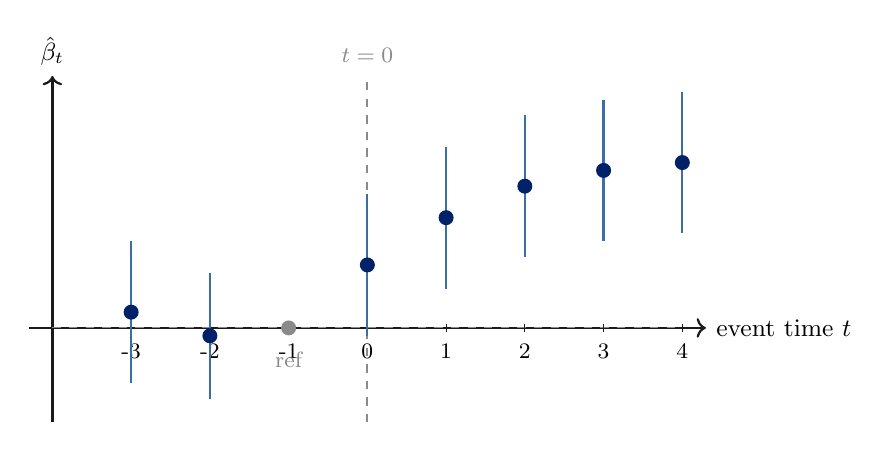
\begin{tikzpicture}
  % Axes
  \draw[->, thick, draw=axes] (-0.3, 0) -- (8.3, 0) node[right] {\small event time $t$};
  \draw[->, thick, draw=axes] (0, -1.2) -- (0, 3.2) node[above] {\small $\hat{\beta}_t$};

  % Horizontal reference line at beta = 0
  \draw[dashed, draw=ref] (0, 0) -- (8, 0);

  % Vertical reference at t = 0 (x = 4)
  \draw[dashed, thick, draw=ref] (4, -1.2) -- (4, 3.2);
  \node[above, ref, font=\footnotesize] at (4, 3.25) {$t = 0$};

  % X-axis tick labels
  \foreach \x/\label in {1/-3, 2/-2, 3/-1, 4/0, 5/1, 6/2, 7/3, 8/4} {
    \draw[draw=axes] (\x, -0.05) -- (\x, 0.05);
    \node[below, font=\footnotesize] at (\x, -0.08) {\label};
  }

  % Confidence intervals and point estimates.
  % \foreach expands (x, est, lo, hi) into a CI bar followed by a point.
  \foreach \x/\est/\lo/\hi in {
    1/0.20/-0.70/1.10,
    2/-0.10/-0.90/0.70,
    4/0.80/-0.10/1.70,
    5/1.40/0.50/2.30,
    6/1.80/0.90/2.70,
    7/2.00/1.10/2.90,
    8/2.10/1.20/3.00
  } {
    \draw[thick, draw=ci] (\x, \lo) -- (\x, \hi);
    \filldraw[point] (\x, \est) circle (2.5pt);
  }

  % Reference period (t = -1, x = 3): zero by construction, no CI.
  \filldraw[ref] (3, 0) circle (2.5pt);
  \node[below, ref, font=\footnotesize] at (3, -0.18) {ref};
\end{tikzpicture}
\end{document}
